\documentclass{mcmthesis}
\mcmsetup{CTeX = false,
        tcn = 2425159, problem = C,
        sheet = true, titleinsheet = true, keywordsinsheet = true,
        titlepage = false, abstract = true}
% \usepackage{newtxtext,newtxmath}
\usepackage{palatino}
\usepackage{lipsum}
\usepackage{algorithm}
\usepackage{algpseudocode}
\usepackage{colortbl}
\usepackage{hhline}
\usepackage{array}
\usepackage{geometry}
\usepackage{graphicx}
\usepackage{amsmath}
\usepackage{amsfonts}

% \usepackage{hyperref}
\title{Tennis Player "Momentum" Prediction}

\begin{document}
\begin{abstract}

\begin{keywords}

\end{keywords}
\end{abstract}
\maketitle
%% Generate the Table of Contents, if it's needed.
 \tableofcontents
 \newpage
%% Generate the Memorandum, if it's needed.


%%\section为一级标题,\subsection为二级标题 \subsubsection为三级标题

\section{Introduction}

\subsection{Problem Background and Literature Review}
\hspace*{1em} In the 2023 Wimbledon Gentlemen's final, the match between Carlos Alcaraz and Novak Djokovic % 
displayed a contest full of uncertainties. From the onset, the seasoned Djokovic seemed to have the upper hand, % 
but the subsequent comeback by Alcaraz showcased the resilience of the young challenger. % 
The alternating lead in sets not only reflected the technical prowess of both players but also hinted at % 
a more elusive element within the match --- a force that subtly alters the course of the game at pivotal moments. \\
\hspace*{1em} This force, commonly understood as the "momentum" of the match, is precisely what infuses each contest % 
with possibilities, sparking interest in the deeper dynamics of sporting competitions.

\subsection{Restatement of the Problem}
\hspace*{1em}Considering the background information %
and additional guidance, we need to solve the following problems:
\begin{itemize}
\item Task1: Develop a model capable of capturing the flow of play as points occur, % 
quantifying player performance during various intervals, and providing a visual representation. %
Additionally, the model must account for the significant advantage of the serving player.
\item Task2: Employ the proposed model to verify whether momentum is a key factor in causing %
swings in the dynamics of a match, determining if changes in the course of the game are random or not.
\item Task3: Develop a predictive model using data from at least one match to forecast when the %
momentum may swings between players in a tennis match. Identify any significant factors that %
correlate with these changes. Then, advise a player on strategy for an upcoming match, %
taking into account historical momentum swings from past games.
\item Task4: Evaluate the model's effectiveness in predicting match momentum swings by %
testing it on additional matches. Assess the accuracy of these predictions, %
identify any shortcomings, and consider what factors might improve future models. %
Determine the model's applicability to different matches.
\end{itemize}

\subsection{Our Work}
\hspace*{1em} Based on the analysis of the problems, we propose the model framework shown in figure 1, %
which is mainly composed of the following parts:

\begin{itemize}
\item We first introduced the Elo rating system based on historical match data (from 2015 to 2023) to quantify the players' inherent %
skills before each match. This player skill level was used as an input for subsequent models, allowing us to incorporate players' %
abilities into our macro-level model. Building upon this foundation, we proposed our macro-level model.....................

\item
\item Expanding on our macro-level model, we introduced a micro-level model that considers detailed match data. %
Our micro-level model focuses on capturing player performance patterns at the point level. This helped us predict %
player points' probabilities more realistically. %
\item By comparing the results of micro-level model and macro-level model, we can forecast player momentum and identify swings in it. %
Additionally, we analyzed this in relation to players' win probability curves to understand how momentum changes %
affected their chances of winning. Using these insights, we could offer personalized recommendations to the players.
\end{itemize}

\begin{figure}[]
\centering
\includegraphics[width=\textwidth]{figures/Business model canvas.pdf}
\caption{Work overview}
\label{fig:businessmodelcanvas}
\end{figure}

\section{Assumptions and Notations}

\subsection{Model Assumptions}
\begin{itemize}
\item
\item
\item
\item
\end{itemize}


\subsection{Notations}
\begin{itemize}
\item
\item
\item
\item
\end{itemize}

\section{Data Preprocessing and Exploratory Analysis}

\hspace*{1em} Besides the official \texttt{Wimbledon\_featured\_matches.csv} dataset, %
we also utilized the \texttt{atp\_matches\_2015.csv} dataset, which includes detailed %
data of all tennis matches in 2015. Prior to developing the model, we need to %
preprocess these datasets. In the initial data of \texttt{Wimbledon\_featured\_matches.csv}, %
we identified several anomalies and missing values.
\begin{itemize}
\item In the \texttt{Wimbledon\_featured\_matches.csv} dataset, we detected anomalies in %
the \texttt{elapsed\_time} column with durations exceeding 24 hours, which we subsequently corrected. %
Additionally, we conducted data cleaning by eliminating 64 records with missing values.
\item In the \texttt{atp\_matches\_2015.csv},
\end{itemize}

\begin{figure}[htbp]
\centering
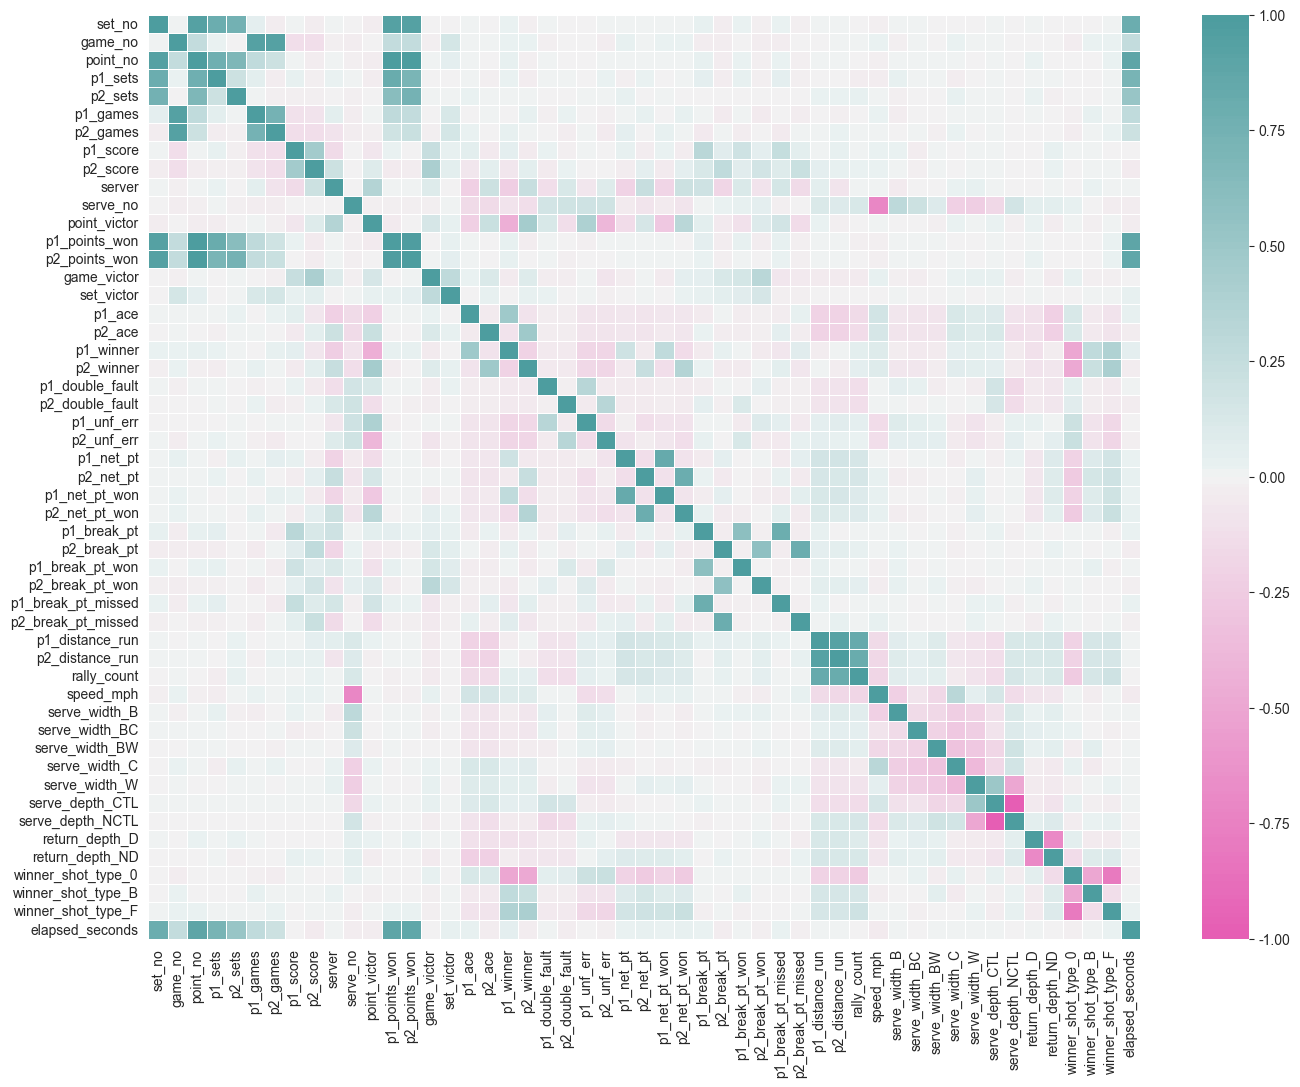
\includegraphics[width=0.7\linewidth]{"figures/heatmap.png"}
\caption{Heatmap}
\label{fig:heatmap}
\end{figure}

\begin{figure}[htbp]
\centering
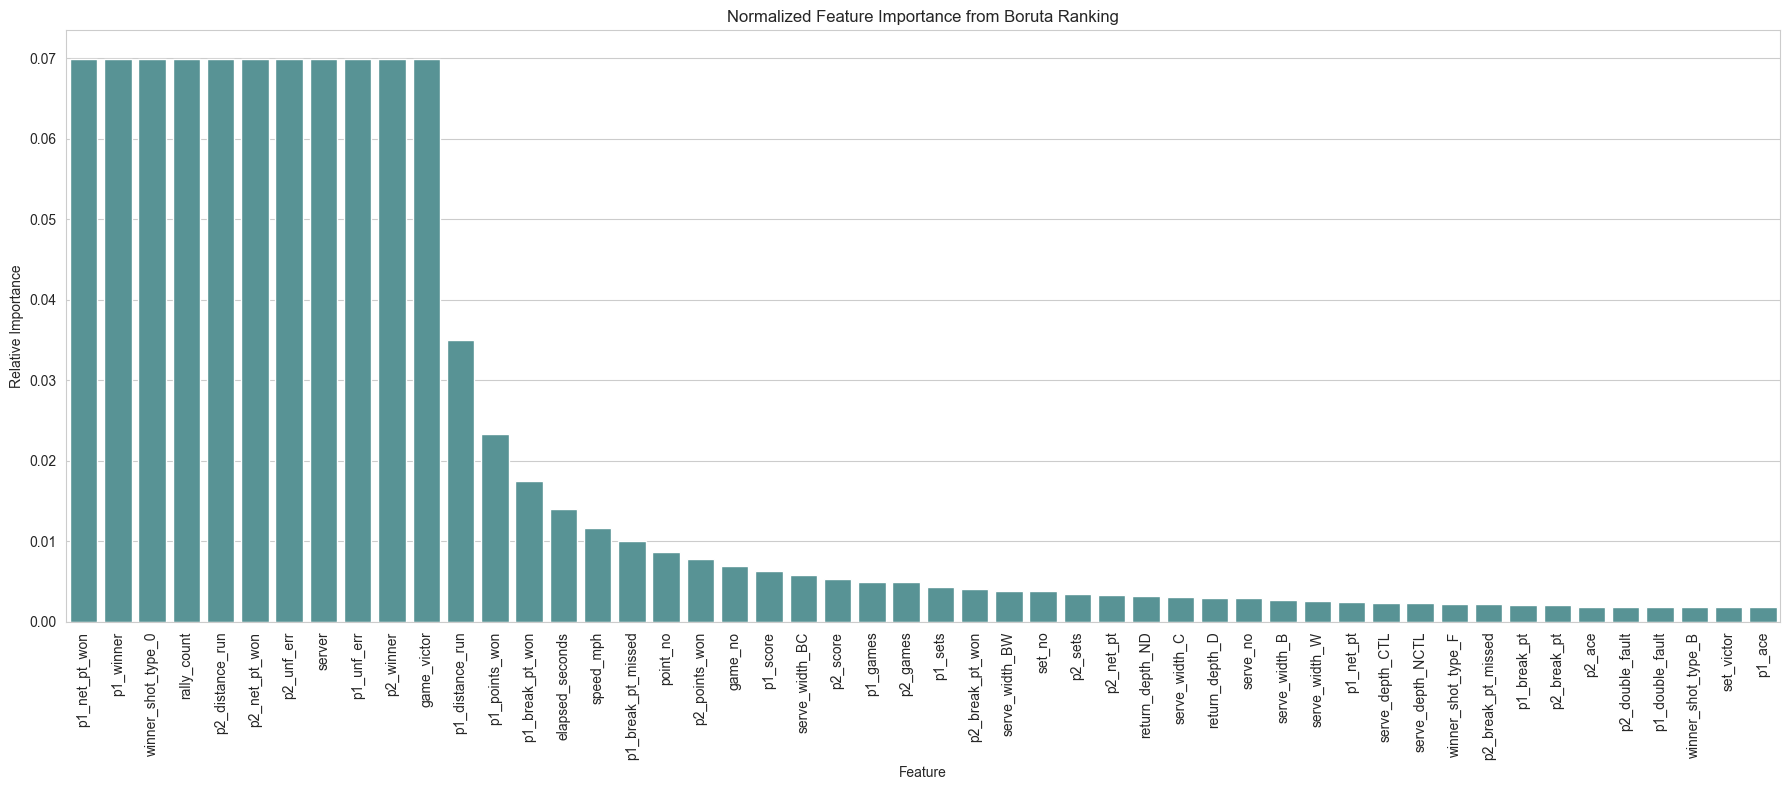
\includegraphics[width=\linewidth]{"figures/boruta of all data.png"}
\caption{Importance Rank}
\label{fig:rank}
\end{figure}

\section{Task1: }

\section{Task2: }
We find the connection between momentum and swings in play from the previous model.%
In this task, we pinpointing break serve as a critical factor. We compare different methods and employ logistic regression, %
enhancing the model's accuracy with K-fold cross-validation and hyper-parameter optimization to probe%
 the relationship between break points and swings in play. This refined approach allows%
  us to substantiate the sequence from momentum through break serve to game swings,%
   thus affirming the strategic significance of momentum in tennis matches.

\subsection{method selection}

When it comes to calculate, we come up with two ideas. Firstly, the whole tennis match can be easily %
transferred to the Hierarchical Markov Model. Because the process strictly follows a level-based %
structure. Winning a point helps you gain one score in this game, and winning a game contributes to the set,etc.
So if we can construct a Hierarchical Markov Model, we can thus predicting one game.% 

We employ logistic regression, enhancing the model's accuracy with K-fold cross-validation and %
hyper-parameter optimization to probe the relationship between break points and fluctuations in %
win probability. 

We can compute the transition probability from player's historical match statistics. In order to %
eliminate the impact of transition probability caused by receiving and serving games, we calculate the %
transition probabilities, which include the probability of Player 1 winning each point in both receiving %
and serving games, and similarly for Player 2: %
\[
  f_{xy} = \frac{\sum N(\text{points of player1 win in serve})}{\sum N(\text{points of player1 in serve})}
\]

Using these probabilities %
and historical data, we construct the Hierarchical Markov Model, starting from the point level and%
  progressing to game, set, and match levels. The model then predicts the winners at these different %
levels based on these probabilities and historical insights. The boundary values for the point-game,game-set%
 set-match layers are as follows:

 point-game:
 \[
  g(x,y)=\begin{cases} 1,&\text{if $x$ >3, $x$-$y$>1}\\
    0,&\text{if $y$ >3, $y$-$x$>1}\\
    f_{x,y} g(x,y-1)+(1-f_{x,y}) g(x-1,y),&\text{if $x$=5 or $y$=5}\\
    f_{x,y} g(x+1,y)+(1-f_{x,y}) g(x,y+1),&\text{otherwise}\\    
  \end{cases}
\]

game-set:
 \[
  s(x, y) = 
  \begin{cases} 
  1, & \text{if } g_1 \geq 6, x - y \geq 2 \\
  0, & \text{if } g_2 \geq 6, x - y \geq 2 \\
  s'(s_1, s_2), & \text{if } g_1 = g_2 = 6 \\
  g(0,0)(1 - s(g_2, g_1 + 1)) + (1 - P_g(0,0))(1 - P_s(g_2 + 1, g_1)), & \text{otherwise}
  \end{cases}
\]

set-match:
\[
  m(x, y) = 
  \begin{cases} 
  1, & \text{if } x \geq 2 \\
  0, & \text{if } y \geq 2 \\
  s(0, 0)m(x+1,y)+(1-s(0,0))m(x,y+1), & \text{otherwise} \\
  \end{cases}
\]

By putting fxy into the point-game layer, we can calculate the win probability of the whole match.%



From previous model we find the momentum may affect the break serve, while break serve is highly related to %
swings in game. So in this task, we try to demonstrate the correlation between momentum and break serve, thus %
showing the swings in play and runs of success by one player are not random.
\subsection{Feature generation}
Generate "lead margin" as heuristic to help the model better measuring the current progress in a competition. 
\[
  H_{xy} = g(x) - g(y) + (p(x)-p(y))/4
\]
We divide p(x)-p(y) by 4 because normally winning 4 points wins this game. 



\subsubsection{markov chain model}
We have established a model based on the tennis rules in the question: a match is divided %
into many layers: match,set,game and point, and winning a match requires winning at least three sets, while winning %
a set requires winning at least six games. The general games (except for the seventh round)%
follows the pattern: the player wins when they reach 4 points, but must win %
 the opponent by an additional 2 points. We still use the AD scores of 0, 15, 30, and 40 in %
 tennis matches for scoring, but use 55 points instead of AD to unify the data type and %
 better fit it into the model for calculation.
Each score has two transition probabilities to represent win or lose, namely the transition probabilities between %
player 1's score and player 2's score. We can easily construct a Markov chain model in %
adjacent layers (point and game, game and set, set and match) based on the win or loss %
of each game: (see Figures 1, 2, 3)

We consider each score X: Y as a state, for example, in each new game, we will start %
from 0:0. When player1 reaches a state of 40:X (X<=30) or 55:40 and wins the next game, he wins each game, and the game set Markov chain model in the previous layer will also enter a new state accordingly. Similarly, in each set, win six or more matches with an advantage of at least two (except for the need to directly determine the winner by grabbing seven at 6:6); The player who wins 2 points in the match and wins the next set wins this game.
Each arrow represents a transition to the state indicated by the arrow. The transition %
between probabilistic states depends on the probability of player1 winning in the current %
state. For example, going from "0,0" to "15,0" may indicate that player A has won one point. %
When the game state is at the end point, the model will pass it to its upper layer %
(game ->set ->match) based on its position. We define its boundary state as:

\subsubsection{Elo forecast model}
The ELO Rating System is a recognized and authoritative rule for assessing the level of %
playing chess today, and has been widely applied in sports and games such as chess, Go, %
football, tennis, and basketball. For each match, it updates its value based on player's performance:

\[
E_{p_i}(m + 1) = E_{p_i}(m) + K_{p_it} \cdot (W_{p_i}(m) - \hat{\pi}_{{p_i}{p_j}}(t))
\]

\(W_i(t)\) is an indicator for whether \(p_i\) won the given match, while \(K_{it}\) is the learning rate %
for \(p_i\) at time \(t\). Since K don't have a definite value, a better value for K can raise its performance%
on prediction.

And in tennis, Five ThirtyEight's Elo variant has raised attention due to its high predictive rate. %
Its main idea is to optimize the formular on learning rate. According to FiveThirtyEight’s analysts, %
Elo ratings perform optimally when allowing Kit to decay slowly over time (Bialik et al., 2016).%
With \(m_i(t)\) representing \(p_i\)'s career matches played at time \(t\) we update our learning rate:

\[
K_{it} = \frac{250}{(5 + m_i(t))^4}
\]

%chaode

Such form of calculating is more sensitive to the data of newcomers who do not have many competitions in career. %
a player’s Elo most quickly when we have no information about a player
and makes smaller changes as mi(t) accumulates. Using this learning rate, we can get to know more about %
a fresh player (just like Carlos Alcaraz, the Champion of Wimbledon, 2023).To apply this Elo rating method to our
dataset, we initalize each player’s Elo rating at Ei(0) = 1500 and match history mi(0) = 0.
Then, we iterate through all tour-level matches from 2013 to 2023 in chronological order, storing
Ei(t), Ej (t) for each match and updating each player’s Elo accordingly. Thus we make use of the %h
historical data from elo to compensate the shortage of data volume

It analyzes historical data and generates %
corresponding elo scores to predict match results. The formular is as follows:

\[
\hat{\pi}_{ij}(t) = \left(1 + 10^{\frac{E_j(t) - E_i(t)}{400}} \right)^{-1}
\]

After we generate the elo score and pre-match prediction win rate, we add the two columns to the corresponding %
matches in data.csv

This provides valuable information about the relative strength of players to our existing %
models, to some extent compensating %
for the prediction errors caused by the lack of model data, and helping us better predict %
the desired results. And its numerical value is single, making it easy to integrate as a %
feature into our various algorithms to provide assistance. In this Elo prediction model, %
we found detailed and high-quality match specific information from the database provided %
by JeffSackmann, and extracted data from all competitions between 2013 and 2023. We %
calculated elo scores for specific player1 and player2, giving elo (p1) and elo (p2), so %
that we can make preliminary predictions on the data before the game.




\section{Task3: }



\subsection{CNN-GRU-Attention Model}

Given an input matrix $X$, representing the time series data, this model aims to capture short-term patterns within the data, %
such as trends in a tennis player's consecutive wins or losses. The model operations are as follows:

1. \textbf{Convolution and GRU Operations}:
\begin{equation}
    X_{\text{gru}} = \text{GRU}(\text{Transpose}(\text{Conv}(X)))
\end{equation}
Where $\text{Conv}(X)$ applies a convolution operation on $X$ to extract local features from the time series, %
and $\text{Transpose}(\cdot)$ prepares the data for sequential processing. $X_{\text{gru}}$ is the output of the GRU layer, %
which captures temporal dependencies in the data.

2. \textbf{Attention Weighted Sum}:
\begin{equation}
    X_{\text{attention}} = \sum_{t=1}^{N} \text{Softmax}\left(\text{Tanh}(W_1 \cdot X_{\text{gru},t} + b_1) \cdot W_2 + b_2\right) \cdot X_{\text{gru},t}
\end{equation}
Where the attention mechanism assigns weights to each time step, emphasizing the most relevant parts of the time series, %
and $X_{\text{attention}}$ is the result of applying these weights, providing a focused representation of the input.

3. \textbf{Batch Normalization and Output Layer}:
\begin{equation}
    P = \text{Sigmoid}\left(W_o \cdot \text{BatchNorm}(X_{\text{attention}}) + b_o\right)
\end{equation}
Where $P$ represents the output probabilities, obtained using the output layer. Batch normalization is applied conditionally %
to stabilize the learning process and improve model performance.

Overall, the CNN-GRU-Attention model effectively captures both local and temporal features in time series data, %
making it particularly suitable for scenarios where understanding short-term patterns is crucial.



\subsection{CNN-GFT-LSTM Model}

Given an input tensor $X$, representing the sequence data, this model aims to capture both spatial and temporal %
patterns within the data, alongside frequency domain characteristics. The model operations are as follows:

1. \textbf{Convolution Layer}:
\begin{equation}
    X_{\text{conv}} = \text{ReLU}(W * X + b)
\end{equation}
Where $W$ and $b$ represent the weights and bias of the convolution layer, respectively, and $\text{ReLU}(\cdot)$ %
ntroduces non-linearity, enhancing the model's ability to learn complex patterns.

2. \textbf{Global Fourier Transform Encoder}:
\begin{equation}
    X_{\text{fft}} = \sqrt{\text{Re}(\text{FFT}(X_{\text{conv}}))^2 + \text{Im}(\text{FFT}(X_{\text{conv}}))^2}
\end{equation}
This operation applies a Fast Fourier Transform (FFT) to $X_{\text{conv}}$, extracting frequency domain features. %
The magnitude of the FFT output, $X_{\text{fft}}$, captures the energy spectrum of the sequence, providing a global %
view of its frequency components.

3. \textbf{LSTM Layer}:
\begin{equation}
    (H_t, C_t) = \text{LSTM}(X_{\text{fft}}[t], (H_{t-1}, C_{t-1}))
\end{equation}
Here, $X_{\text{fft}}[t]$ is the input at time step $t$, and $(H_t, C_t)$ represent the hidden and cell states at time step $t$, %
respectively. The LSTM layer processes the sequence one step at a time, updating its state based on both the current input and the %
previously accumulated information.

4. \textbf{Linear Layer and Sigmoid Activation}:
\begin{equation}
    P = \text{Sigmoid}(W_{\text{fc}}H_T + b_{\text{fc}})
\end{equation}
Where $W_{\text{fc}}$ and $b_{\text{fc}}$ are the weights and bias of the fully connected layer, respectively, %
and $H_T$ is the hidden state from the last time step of the LSTM. The Sigmoid function is applied to obtain the final prediction $P$, %
mapping the output to a $(0, 1)$ range suitable for binary classification tasks.
Overall, the CNN-GFT-LSTM Model effectively integrates convolutional, Fourier transform, and recurrent neural network mechanisms, %
enabling it to capture spatial, frequency, and temporal dependencies within sequence data. This makes it particularly adept for %
tasks requiring nuanced understanding of such data, such as signal processing or time series forecasting.



\subsection{Integrated Model}
Given the outputs from the CNN-GRU-Attention model, $P_{\text{CGA}}$, and the CNN-GFT-LSTM model, $P_{\text{CGL}}$, %
the integrated model combines these to leverage both short-term and long-term, including cyclical, pattern recognition capabilities. %
The combined prediction, $P_{\text{combined}}$, is computed as:

\begin{equation}
P_{\text{combined}} = \alpha \cdot P_{\text{CGA}} + (1 - \alpha) \cdot P_{\text{CGL}}
\end{equation}
where $\alpha$ is a weight factor between 0 and 1 that balances the contribution of each model to the final prediction.

The integrated model offers a flexible and adaptable approach to capturing a comprehensive range of patterns in time series data. %
By adjusting the weight factor $\alpha$, it seamlessly balances between emphasizing short-term dynamics captured by the CNN-GRU-Attention %
model and the long-term, spatial, and frequency domain insights provided by the CNN-GFT-LSTM model. This combination not only enhances %
the model's overall prediction accuracy and robustness but also ensures a more nuanced understanding of the data's underlying patterns. %
The ability to adjust $\alpha$ allows for the optimization of the model's performance across various datasets and tasks, making it %
particularly suitable for complex time series forecasting challenges.

\begin{figure}[htbp]
\centering
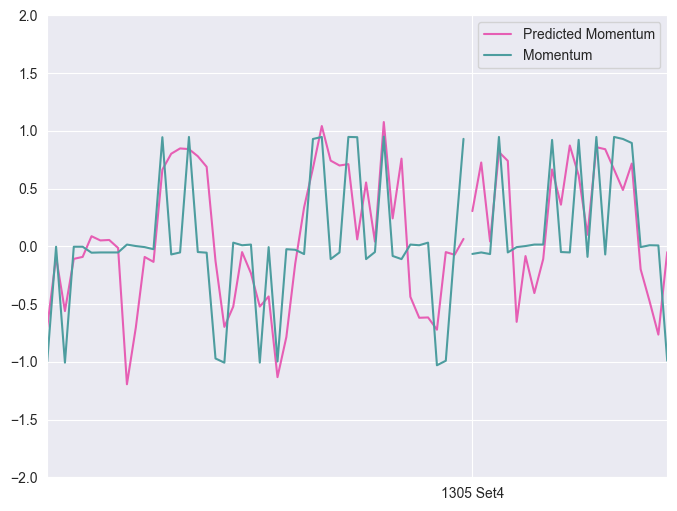
\includegraphics[width=\linewidth]{"figures/predicted momentum vs momentum.png"}
\caption{Predicted Momentum vs Momentum}
\label{fig:pvm}
\end{figure}

\begin{figure}[htbp]
\centering
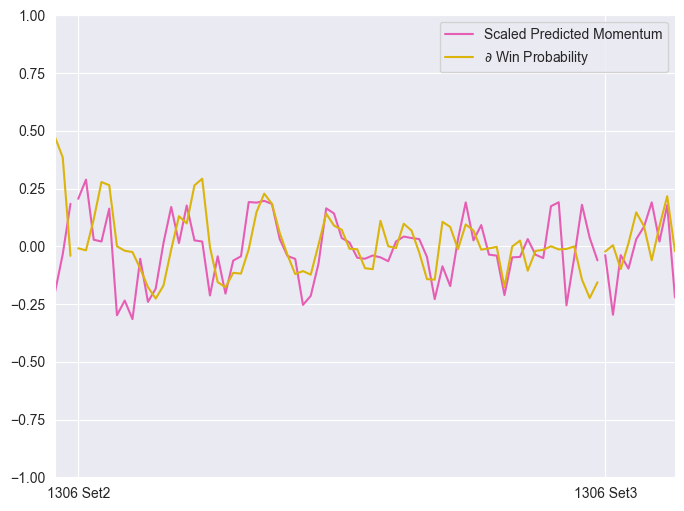
\includegraphics[width=0.5\linewidth]{"figures/predicted momentum vs partial win probaility.png"}
\caption{Predicted Momentum vs Partial Win Probability}
\label{fig:pmvpp}
\end{figure}

\section{Task4: }

\section{Strengths and Weaknesses}

\subsection{Strengths}

\subsection{Weaknesses}

\begin{thebibliography}{99}
% \bibitem{1} D.~E. KNUTH   The \TeX{}book  the American
% Mathematical Society and Addison-Wesley
% Publishing Company , 1984-1986.
% \bibitem{2}Lamport, Leslie,  \LaTeX{}: `` A Document Preparation System '',
% Addison-Wesley Publishing Company, 1986.
% \bibitem{3}\url{http://www.latexstudio.net/}
% \bibitem{4}\url{http://www.chinatex.org/}
\end{thebibliography}

\begin{appendices}

\section{First appendix}

\section{Second appendix}

\end{appendices}

\end{document}